\documentclass[]{beamer}
%\usepackage{beamerarticle}
\usepackage{tikz}
\usetikzlibrary{arrows,shapes}
\author{S. Poss}
\title{From high energy physics to web development}
\subtitle{A tale of a change}

\mode<presentation>
{
  \usetheme{Singapore}
   \setbeamertemplate{navigation symbols}{}
   \setbeamertemplate{footline}[frame number] 
}

\AtBeginSection[]
{
\begin{frame}<beamer>
\frametitle{Outline}
\tableofcontents[currentsection,currentsubsection]
\end{frame}
}


\begin{document}
\begin{frame}
\titlepage
\end{frame}

\begin{frame}
\frametitle{Outline}
\tableofcontents
% You might wish to add the option [pausesections]
\end{frame}

\begin{frame}
\frametitle{Disclaimer}
\centering
Everything here is only my point of view and does not reflect a generality!
\end{frame}

\section{Personal background}
\begin{frame}
\frametitle{2000 - 2009: Particle physics}
\begin{itemize}
\item My initial passion
\item Romantic view of the domain
\item Believed I would get a Nobel prize
\end{itemize}
$\Rightarrow$ PhD.: CP violation in LHCb
\pause
\begin{itemize}
\item Realized something was off
\item More interested in the tools than in the science
\item More fun doing computing thing
\end{itemize}
\end{frame}

\begin{frame}
\frametitle{2010 - 2013: The CERN years}
\begin{itemize}
\item Huge opportunity to work in my dream lab
\item Project for the future
\item Amazing people
\item Amazing place
\end{itemize}
\pause
But:
\begin{itemize}
\item Every good things end
\item Didn't see myself move again
\end{itemize}
\end{frame}

\begin{frame}
\frametitle{May 2013 - December 2013: Self-employed}
\begin{itemize}
\item Opportunity to work for CERN as self-contractor
\item Pocket money
\item Looking for 'real' jobs
\item Lazy
\end{itemize}
Doubt about future settles in
\end{frame}

\begin{frame}
\frametitle{Dec. 2013 - 2015: Alpes Lasers, NOTEDEV}
\begin{itemize}
\item Job ad. fitted my profile: Expert in distributed computing
\item Place not far from where I lived
\item New domain: interesting challenges
\item Industry!
\end{itemize}
\pause
Issues:
\begin{itemize}
\item 3 months to complete initial objective
\item System never used
\item Did not do what I was hired for
\item Depression
\end{itemize}
Was offered contract extension but refused
\end{frame}

\begin{frame}
\frametitle{2016 - ?: Xample Sarl, web developer}
\begin{itemize}
\item June to December: $\approx 10$ job applications, 3 interviews
\item Day I left Alpes: interview
\item Contract signed 8 days after
\item Started in January
\end{itemize}
\pause
So far:
\begin{itemize}
\item I belong there
\item It's interesting/challenging
\item I won't do that for the rest of my life
\end{itemize}
\end{frame}

\section[Differences]{Differences between research and industry}
\begin{frame}
\frametitle{The differences}
\begin{itemize}
\item Money
\item Strict deadlines
\item Customer relations
\item Timing
\item Technical aspects
\end{itemize}
\end{frame}

\section[Motivations]{The motivations to change}
%\begin{frame}
%\frametitle{Motivations to move on}
%\begin{itemize}
%\item No job
%\item Lack of mobility
%\begin{itemize}
%\item Family
%\item Location
%\end{itemize}
%\item Lack of faith
%\item Not what you thought it was
%\begin{itemize}
%\item management, projects, grant applications
%\end{itemize}
%\end{itemize}
%\end{frame}
%
%\begin{frame}
%\centering
%\Huge{\color{blue}{The reasons to move away from research}}
%\end{frame}

\begin{frame}
\centering

\includegraphics[width=0.6\textwidth]{No-Vacancy-Sign}

Number of post-doc position are dropping, worst for tenure-track positions
\end{frame}

\begin{frame}
\centering
\begin{columns}
\column{0.45\textwidth}
\centering

\includegraphics[width=\textwidth]{family}
\column{0.45\textwidth}
\centering
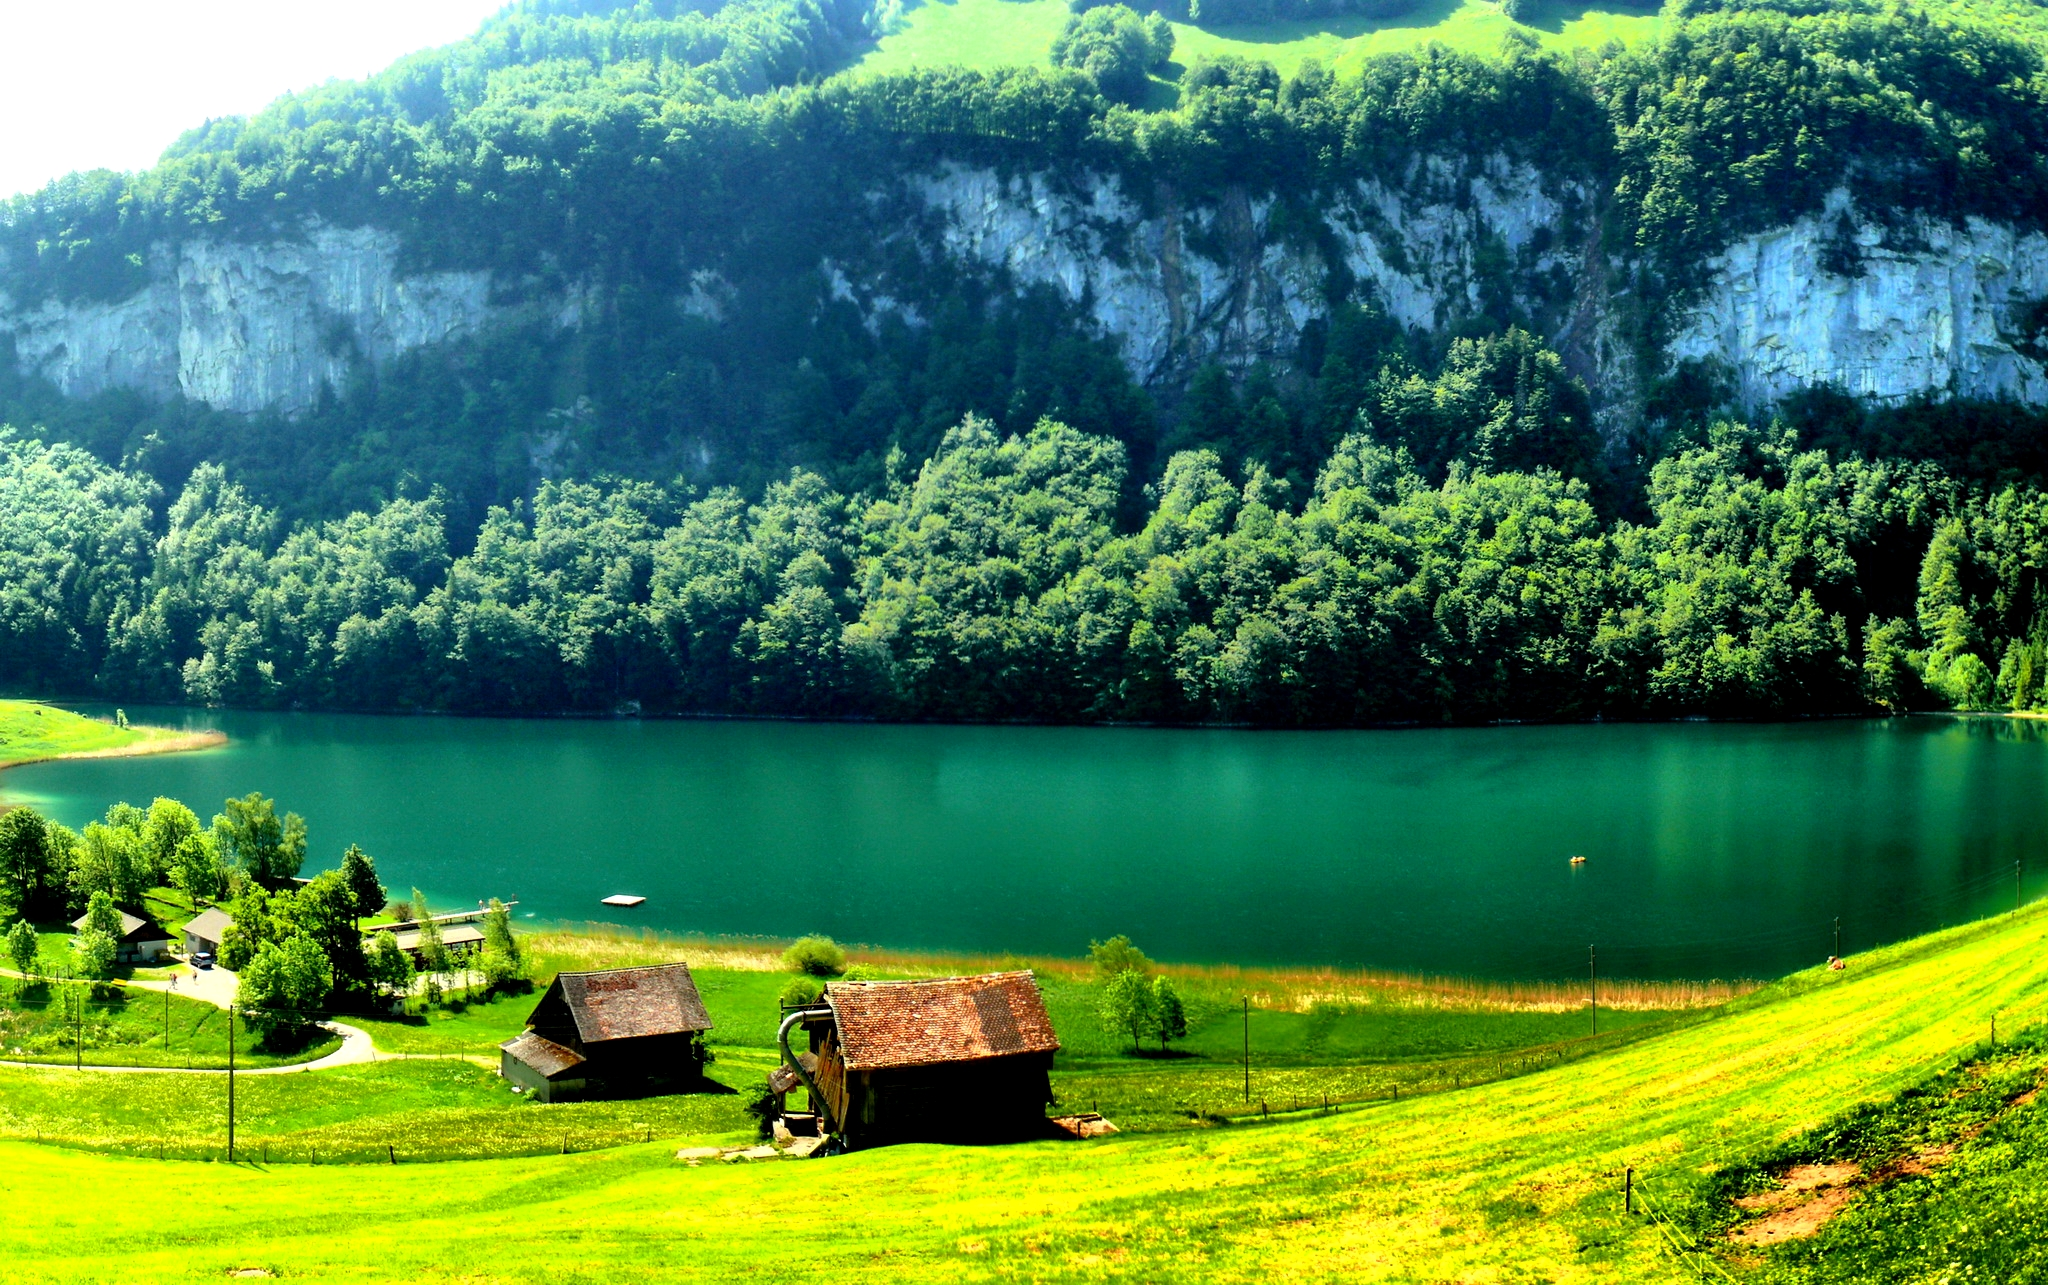
\includegraphics[width=\textwidth]{beautiful-place}

\end{columns}
\end{frame}

\begin{frame}
\centering
You don't believe in what you do
\end{frame}

\begin{frame}
\centering
Research is not what you thought it was
\end{frame}

\section[Questions]{Questions for you}
\begin{frame}
\frametitle{Some questions to ask yourself}
\begin{itemize}
\item Am I the kind of person who values intellectual freedom more than financial security? \pause
\item Do I really love the process of actually doing science enough to warrant investing a huge amount of my time and energy over the next few years? \pause
\item Can I deal with perpetual uncertainty about my future? \pause
\item And ultimately, would I be okay doing something that I really enjoy for N years if at the end of that time I have to walk away and do something very different?
\end{itemize}
\end{frame}

\section{Worries}
\begin{frame}
\frametitle{Some worries you may have}
\begin{itemize}
\item Is what you did relevant?\pause \quad \alert{Yes} \pause
\item Will you find a job?
\end{itemize}
\end{frame}

\begin{frame}
Unemployment rate for former PhDs.: 2\%
\centering
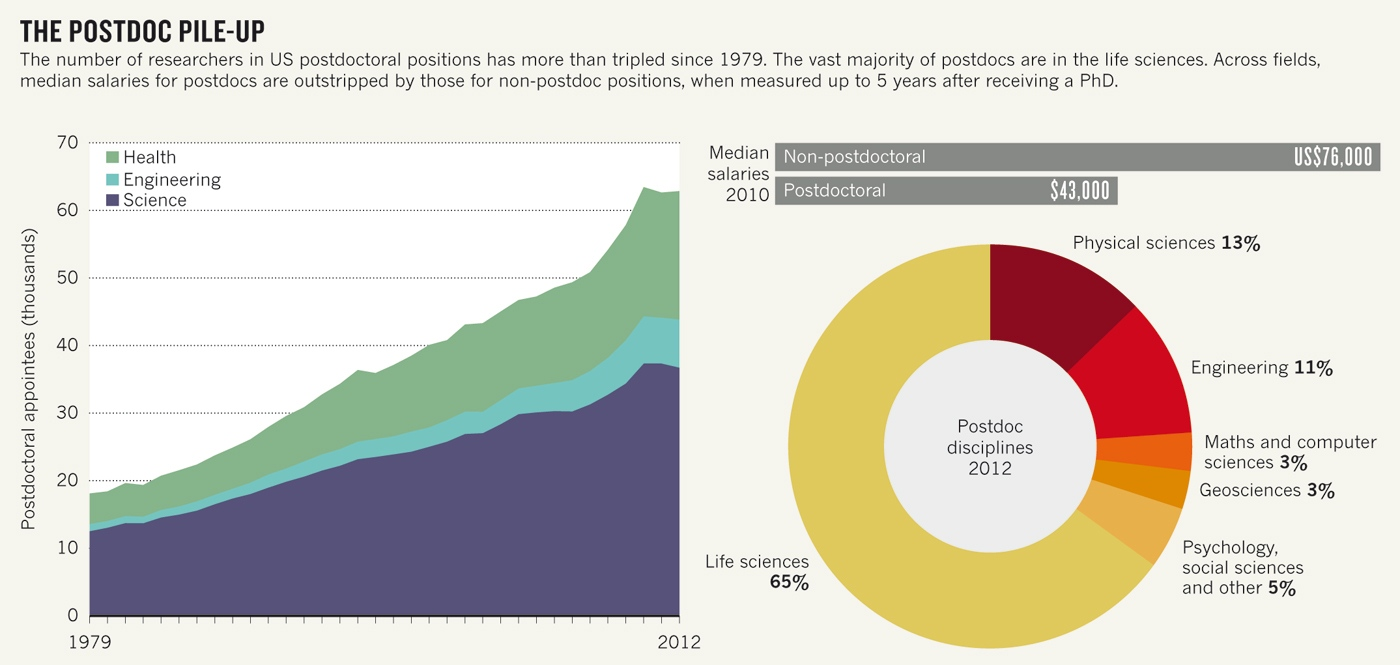
\includegraphics[width=0.9\textwidth]{Postdoc2}
\end{frame}

\begin{frame}
\centering
61\% of people with STEM degree have careers outside academia
\end{frame}

\section{Risks}
\begin{frame}
\frametitle{What you could face}
\begin{itemize}
\item Lots of stress
\item Depression
\end{itemize}\pause
What you can do:
\begin{itemize}
\item Start new activities
\item Keep seeing friends
\item See a therapist to help coping with the doubt
\end{itemize}
\end{frame}

\begin{frame}
\centering

\includegraphics[width=\textwidth]{just_then}
\end{frame}

\end{document}